\section{Restoring Force Surface}
\label{sec:rfs_description}

The restoring force surface (RFS) method, introduced by \parencite{masri1979a}
and covered in details in \autocite{worden1990a}, have previously been used as a
parameter estimation technique, but is only used as a visual tool for
characterization the functional form of the nonlinearity in this report.

If RFS is used for parameter estimation, an estimation of the inertia for the
system is needed. This either requires an FE model or, for more than a few DOFs,
an complicated algebraic model.

The starting point is Newton's second law of written for a specific DOF located
next to a nonlinear structural component

\begin{equation}
  \label{eq:rfs_newton}
  \sum_{k=1}^{n} m_{i,k} \ddot x_k + f_i(\bm x, \dot{ \bm x}) = p_i
\end{equation}
where $i$ is the DOF of interest, $n$ the number of DOFs in the system, $m_{ik}$
the mass matrix elements, $\bm x$, $\dot{\bm x}$ and $\ddot{ \bm x}$ the
displacement, velocity and acceleration vectors, respectively, $\bm f$ the
restoring force vector encompassing elastic and dissipative effects, and $\bm p$
the external force vector.

Let $j$ denote another measured DOF located across the nonlinear connection, see
figure \ref{fig:rfs_schematic}, a new formulation of \eqref{eq:rfs_newton},
which accounts for the difference in displacement and velocity between the
selected DOFs, is approximated with

\begin{equation}
  \label{eq:rfs_newton2}
  m_{i,i} \ddot x_i +  f_i (x_i - x_j , \dot x_i - \dot x_j) \approx p_i
\end{equation}
where all inertia and restoring force contributions not related to the nonlinear
component are discarded.

\begin{figure}[ht!]
  \centering
  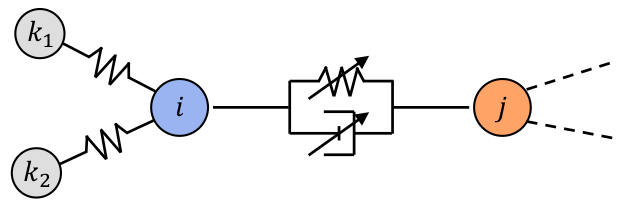
\includegraphics[width=0.5\textwidth]{rfs/rfs_schematic.png}
  \caption{Nonlinear connection between node $i$ and $j$. The linear connections
    $k_{1,2}$ are discarded.}
  \label{fig:rfs_schematic}
\end{figure}

It is further assumed that no external force is applied directly at DOF $i$
(eg. the external force is applied at a different location on the structure), a
rearrangement leads to
\begin{equation}
  \label{eq:rfs}
  f_i (x_i - x_j , \dot x_i - \dot x_j) \approx -m_{i,j} \ddot x_i
\end{equation}

Thus by dropping the constant mass, the nonlinearities can be visualized as the
negative acceleration at one side of the connection, as a function of the
relative displacement and velocity across this connection. From this an adequate
mathematical model can be found.

The shape of $f$ is visualized by plotting the triplet $(x_{i} - x_{j}, \dot
x_{i} - \dot x_{j}, \ddot x_{i})$ The form of elastic (dissipative)
nonlinearities in the connection is visualized by making a slice along the axis
of the zero velocity (displacement) of the restoring force surface plot. Either
prior knowledge about the physics or a least square fit can be used to find the
functional that best represent the nonlinearity.

%The velocity and displacement are found by numerical integration, see section
%\ref{chap:signals}.


The advantages of RFS as presented here, is that it relies exclusively on measured
time series and have a visual understanding. It is not commonly used for
parameter estimation for MDOF systems, due to the need for direct fitting of
Newton's second law.
RFS is also called Accelerated Surface Method (ASM) at times in literature.


The major limitations of the RFS method in general is
\begin{itemize}
\item Requires the nonlinear dynamics to be excited
\item Shows the total restoring force:
  \begin{itemize}
  \item with multiple nonlinearities it is not possible to distinguish them
    uniquely.
  \item If the nonlinear force is of the same magnitude as the linear force, it
    might be necessary to remove a linear trend from the RFS to visualise the
    nonlinear force.
  \end{itemize}
\item Works best swept-sine excitation.
\item Damping characterisation is difficult due to the low numerical magnitude.
\end{itemize}


\subsection{Example}
\label{sec:rfs_example}

Using a sine sweep excitation on the coupled duffing system \eqref{eq:2dof} and
the RFS methodology,
\begin{equation}
  \label{eq:rfs_tol}
  f_i (x_i - x_j , \underbrace{\dot x_i - \dot x_j}_\text{<tol}) \approx - \ddot x_i
\end{equation}
where \textit{tol} determines the slice thickness, the restoring force is
visualised in figs \ref{fig:rfs_full} and \ref{fig:rfs_stiff} for $x_0$ and
$x_1$. A hardening stiffness is seen, without any offset, which correspond to a
uneven nonlinear polynomial stiffness. In this case a third order polynomial for
both DOFs.

\begin{figure}[!ht]
  \centering
  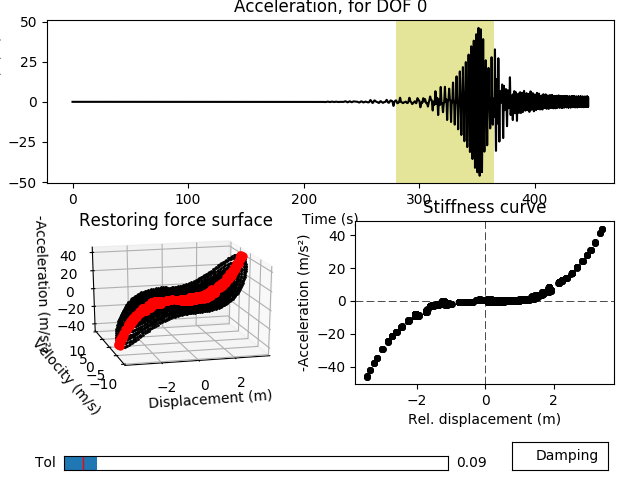
\includegraphics[width=0.8\textwidth]{rfs/sweepvrms3dof0_rfs.png}
  \caption{Interface for selecting the part of the signal used for
    visualising the restoring force of the coupled duffing system
    \eqref{eq:2dof}. Here shown for $x_1$.
    \textbf{upper}: The relevant part of the signal is selected by dragging or
    resizing the yellow rectangle;
    \textbf{left}: Restoring force surface for the selected part of the signal.
    The red line shows the slice;
    \textbf{right}: The visualised stiffness. The slice thickness can be changed
    by dragging the tolerance slider. Damping is visualised by clicking on
    \texttt{damping}.
  }
  \label{fig:rfs_full}
\end{figure}


\begin{figure}[!ht]
  \centering
  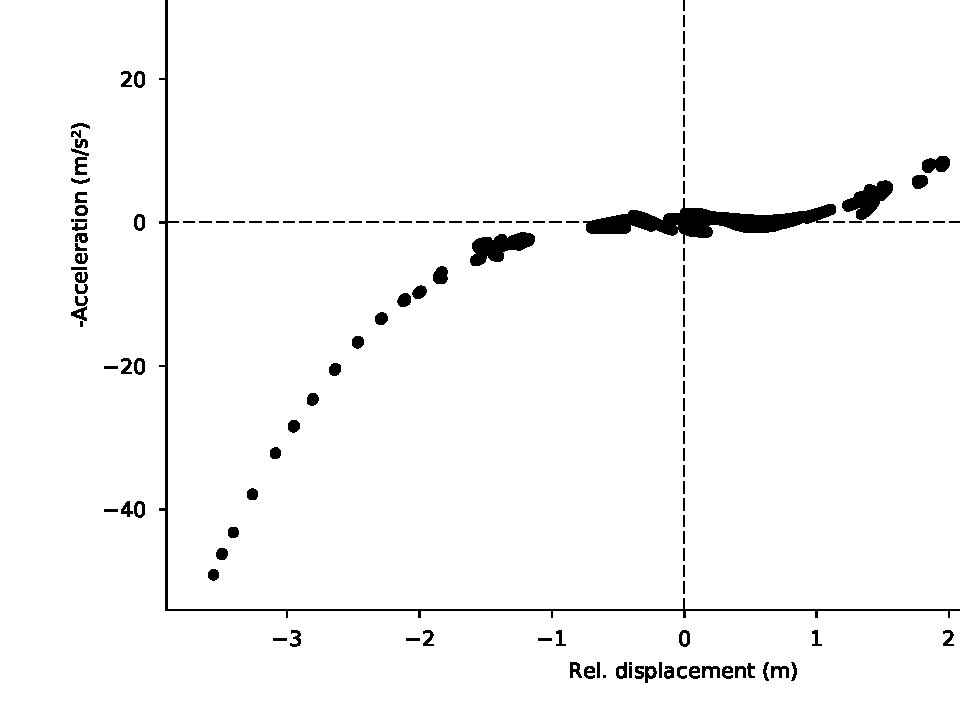
\includegraphics[width=0.6\linewidth, height=6cm]{rfs/sweepvrms3dof1_stiff}
  \caption{The visualised stiffness for $x_2$ from the coupled duffing system
    \eqref{eq:2dof}.
    The figure is extracted from the interface shown in fig. \ref{fig:rfs_full};
    just for $x_2$ instead}
  \label{fig:rfs_stiff}
\end{figure}

\subsection{Summary}
\label{sec:rfs_summary}

The RFS provides a direct visualization of the nonlinear stiffness and, to
lesser extend, damping curve using a SDOF simplification of the EOMs. The steps
are:
\begin{itemize}
\item Instrument the nonlinear connection with two accelerometers and use swept
  sine excitation.
\item Integrate and filter to obtain displacement and velocity.
\item Calculate the 3D acceleration surface over a single connection.
\item Make surface slides to obtain stiffness and damping curve.
\end{itemize}

The success of parameter estimation step is conditional upon an accurate
characterization of all observed nonlinearities.



%%% Local Variables:
%%% mode: latex
%%% TeX-master: "../../report"
%%% End:
